\documentclass[12pt]{article}

% Paquetes básicos
\usepackage[utf8]{inputenc}
\usepackage[T1]{fontenc}
\usepackage[spanish]{babel}
\usepackage{amsmath, amssymb, amsthm}
\usepackage{geometry}
\usepackage{setspace}
\usepackage{array}
\usepackage{booktabs}
\usepackage{hyperref}
\usepackage{graphicx}

% Configuración de página
\geometry{letterpaper, margin=2.5cm}
\setstretch{1.3}

\begin{document}

% Portada
\begin{titlepage}
    \centering

    {\Large Universidad Nacional Autónoma de México\par}
    \vspace{0.5cm}
    {\Large Facultad de Estudios Superiores Acatlán\par}

    \vspace{2cm}

    {\Huge \textbf{El movimiento browniano a través de Fourier}\par}

    \vspace{0.5cm}

    {\Large \textbf{La construcción de Wiener, la ley del logaritmo iterado y su relación con Khinchin}\par}

    \vspace{2cm}

    {\Large \textbf{Integrantes:}\par}
    \vspace{0.3cm}
    {\Large Albor Saucedo Dylan\par}
    {\Large Garcia Rodriguez Lazaro Isaac\par}

    \vspace{0.7cm}

    {\Large \textbf{Materia:} Procesos Estocásticos\par}
    \vspace{0.5cm}

    {\Large \textbf{Profesor:} Julio César Galindo López\par}
    \vspace{0.5cm}

    {\Large \textbf{Fecha:} 22 de mayo de 2026\par}

    \vfill
\end{titlepage}

\tableofcontents
\newpage

\section{Introducción}

El movimiento browniano es uno de los objetos más importantes dentro de la teoría moderna de la probabilidad y de los procesos estocásticos. Su relevancia se debe a que une ideas provenientes de la física, el análisis matemático, la teoría de la medida y la estadística. Aunque originalmente surgió como una observación experimental relacionada con el movimiento irregular de partículas suspendidas en un fluido, con el paso del tiempo se convirtió en un modelo matemático fundamental para describir fenómenos aleatorios continuos.

Desde un punto de vista físico, el movimiento browniano describe el desplazamiento irregular de una partícula pequeña que recibe impactos constantes de moléculas invisibles del medio que la rodea. Sin embargo, desde el punto de vista matemático, este movimiento puede entenderse como un proceso estocástico continuo con incrementos independientes y distribuidos normalmente. Esta transición, de una observación física a una formulación matemática rigurosa, representa uno de los momentos más importantes en la historia de la probabilidad.

En el video de Yuval Peres, \textit{Some highlights from the history of probability}, se muestra cómo la probabilidad se fue desarrollando a partir de problemas concretos hasta convertirse en una teoría capaz de explicar fenómenos complejos. El movimiento browniano forma parte de esta evolución porque muestra cómo una idea física puede convertirse en una estructura matemática profunda.

El objetivo de este trabajo es estudiar el movimiento browniano desde tres enfoques principales. Primero, se presenta su origen histórico y su definición matemática. Después, se explica la construcción de Wiener mediante series de Fourier, una idea que permite representar el movimiento browniano como una suma infinita de ondas aleatorias. Finalmente, se analiza la ley del logaritmo iterado y su relación con Khinchin, mostrando cómo las fluctuaciones extremas del movimiento browniano siguen una escala matemática precisa.

La idea central del trabajo es que el movimiento browniano, aunque parece caótico e impredecible, posee una estructura matemática muy rica. Wiener permite construirlo rigurosamente mediante herramientas del análisis, mientras que la ley del logaritmo iterado permite comprender el tamaño de sus fluctuaciones extremas.

\section{Antecedentes históricos del movimiento browniano}

El movimiento browniano recibe su nombre del botánico Robert Brown, quien en 1827 observó al microscopio el movimiento irregular de partículas de polen suspendidas en agua. Brown notó que estas partículas se movían de forma errática, sin una dirección aparente. En un inicio, este fenómeno no fue entendido completamente, ya que no se conocía con precisión la causa de dicho movimiento.

Décadas después, Albert Einstein explicó el movimiento browniano como consecuencia de los choques microscópicos entre las partículas visibles y las moléculas del fluido. Esta explicación fue fundamental porque conectó el fenómeno con la existencia de moléculas y átomos, además de introducir una interpretación probabilística del movimiento.

El trabajo de Einstein permitió comprender que el movimiento observado no era causado por una fuerza externa visible, sino por una gran cantidad de impactos microscópicos aleatorios. Esta idea abrió la puerta al uso de modelos probabilísticos para describir fenómenos físicos. Así, el movimiento browniano se convirtió en una evidencia importante de la naturaleza molecular de la materia y en un problema central para la probabilidad.

Posteriormente, Norbert Wiener dio una formulación matemática rigurosa del movimiento browniano. Antes de Wiener, el movimiento browniano se entendía principalmente desde una perspectiva física. Wiener logró construirlo como un proceso estocástico bien definido, con trayectorias continuas y propiedades probabilísticas precisas. Por esta razón, el movimiento browniano también se conoce como proceso de Wiener.

Dentro de la historia de la probabilidad, el movimiento browniano representa un cambio importante: la probabilidad ya no se limitaba al estudio de eventos discretos, como lanzamientos de dados o juegos de azar, sino que comenzaba a estudiar fenómenos continuos y funciones aleatorias completas.

\section{Procesos estocásticos y movimiento browniano}

Un proceso estocástico es una familia de variables aleatorias indexadas por un parámetro, generalmente el tiempo. Se puede escribir como:

\[
\{X(t): t \in T\},
\]

donde $T$ representa el conjunto de tiempos. Si $T$ es un conjunto discreto, como los números naturales, se habla de un proceso en tiempo discreto. Si $T$ es un intervalo continuo, como $[0,\infty)$, se habla de un proceso en tiempo continuo.

El movimiento browniano es un proceso estocástico en tiempo continuo. Esto significa que para cada instante $t \geq 0$, existe una variable aleatoria $B(t)$ que representa la posición de la partícula en ese tiempo. La trayectoria completa del proceso es una función aleatoria:

\[
t \mapsto B(t).
\]

A diferencia de una variable aleatoria individual, el movimiento browniano no describe solamente un resultado aislado, sino una evolución completa en el tiempo. Cada realización del proceso produce una trayectoria distinta.

\section{Definición matemática del movimiento browniano}

Un proceso estocástico $\{B(t):t\geq 0\}$ se llama movimiento browniano estándar si cumple las siguientes propiedades:

\begin{enumerate}
    \item $B(0)=0$.
    \item Tiene incrementos independientes.
    \item Para $0\leq s<t$, el incremento $B(t)-B(s)$ sigue una distribución normal con media cero y varianza $t-s$:
    \[
    B(t)-B(s)\sim N(0,t-s).
    \]
    \item Sus trayectorias son continuas casi seguramente.
\end{enumerate}

La primera propiedad indica que el proceso comienza en el origen. La segunda señala que lo que ocurre en intervalos de tiempo separados no depende entre sí. La tercera propiedad establece que los incrementos del proceso son normales y que su variabilidad depende únicamente de la longitud del intervalo de tiempo. Finalmente, la cuarta propiedad indica que las trayectorias no presentan saltos.

Para cada $t\geq 0$, se cumple que:

\[
E[B(t)] = 0
\]

y

\[
Var(B(t)) = t.
\]

Esto significa que, en promedio, el proceso se mantiene centrado en cero, pero su dispersión aumenta conforme pasa el tiempo. Mientras mayor sea $t$, mayor será la variabilidad posible de $B(t)$.

Además, la covarianza del movimiento browniano estándar está dada por:

\[
Cov(B(s),B(t))=\min(s,t).
\]

Esta propiedad es muy importante porque caracteriza la dependencia entre los valores del proceso en distintos tiempos.

\section{Interpretación como límite de caminatas aleatorias}

Una forma intuitiva de entender el movimiento browniano es mediante una caminata aleatoria. En una caminata aleatoria simple, una partícula se mueve paso a paso hacia la derecha o hacia la izquierda con cierta probabilidad. Por ejemplo, se puede definir:

\[
X_i=
\begin{cases}
1, & \text{con probabilidad } \frac{1}{2},\\
-1, & \text{con probabilidad } \frac{1}{2}.
\end{cases}
\]

Entonces la posición después de $n$ pasos se puede escribir como:

\[
S_n=X_1+X_2+\cdots+X_n.
\]

Si los pasos se hacen cada vez más pequeños y más frecuentes, la caminata aleatoria se aproxima a un proceso continuo. Bajo una normalización adecuada, este límite es el movimiento browniano.

La normalización típica consiste en considerar:

\[
\frac{S_n}{\sqrt{n}}.
\]

Esta expresión aparece naturalmente en el teorema central del límite. En términos generales, el teorema central del límite afirma que la suma normalizada de muchas variables aleatorias independientes tiende a una distribución normal. El movimiento browniano puede entenderse como una versión funcional de esta idea, donde no solo se estudia el valor final de la suma, sino toda la trayectoria acumulada.

De esta manera, el movimiento browniano puede interpretarse como el límite continuo de una caminata aleatoria discreta. Esta interpretación ayuda a conectar el proceso de Wiener con modelos más simples de pasos aleatorios.

\section{Series de Fourier: idea general}

Antes de explicar la construcción de Wiener, es conveniente recordar brevemente qué es una serie de Fourier. Una serie de Fourier permite representar ciertas funciones como sumas infinitas de senos y cosenos. De manera general, una función periódica puede escribirse como:

\[
f(t)=a_0+\sum_{n=1}^{\infty}\left(a_n\cos(nt)+b_n\sin(nt)\right),
\]

donde los coeficientes $a_n$ y $b_n$ determinan cuánto aporta cada frecuencia a la función.

La importancia de las series de Fourier es que permiten descomponer una función en ondas simples. Cada término de la serie representa una oscilación de cierta frecuencia. Al sumar muchas oscilaciones, se pueden construir funciones muy complejas.

En el contexto del movimiento browniano, Wiener utiliza una idea parecida, pero con una diferencia fundamental: los coeficientes de la serie ya no son números fijos, sino variables aleatorias. Por lo tanto, la suma resultante no produce una función determinista, sino una función aleatoria.

\section{La construcción de Wiener mediante Fourier}

Norbert Wiener construyó el movimiento browniano de forma rigurosa utilizando herramientas del análisis y de la probabilidad. Una manera de entender esta construcción es mediante series aleatorias relacionadas con Fourier.

La idea principal es representar el movimiento browniano como una suma infinita de funciones trigonométricas con coeficientes aleatorios. De forma conceptual, se puede escribir:

\[
B(t)=\sum_{n=1}^{\infty} Z_n\phi_n(t),
\]

donde:

\begin{itemize}
    \item $Z_n$ son variables aleatorias normales independientes.
    \item $\phi_n(t)$ son funciones deterministas relacionadas con una base de Fourier.
    \item La suma infinita genera una trayectoria aleatoria.
\end{itemize}

Una forma más precisa de una expansión tipo Fourier para el movimiento browniano en el intervalo $[0,\pi]$ es:

\[
B(t)=\frac{t}{\sqrt{\pi}}Z_0+\sqrt{\frac{2}{\pi}}\sum_{n=1}^{\infty}Z_n\frac{\sin(nt)}{n},
\quad 0\leq t\leq \pi,
\]

donde $Z_0,Z_1,Z_2,\dots$ son variables aleatorias normales estándar independientes.

Esta expresión muestra que el movimiento browniano puede verse como una suma de una parte lineal aleatoria y una suma infinita de senos con coeficientes aleatorios. El factor $\frac{1}{n}$ hace que las frecuencias más altas tengan menor peso, lo cual ayuda a que la serie converja y produzca trayectorias continuas.

La razón por la que esta construcción funciona está relacionada con la covarianza. Para que el proceso sea un movimiento browniano estándar, debe cumplirse que:

\[
Cov(B(s),B(t))=\min(s,t).
\]

La serie anterior está diseñada precisamente para que la covarianza del proceso construido coincida con esta expresión. En otras palabras, las funciones seno y los coeficientes aleatorios se combinan de tal manera que el resultado tiene la estructura de dependencia correcta.

De manera intuitiva, se puede decir que:

\[
\text{Movimiento browniano}
=
\text{suma infinita de ondas aleatorias}.
\]

Cada término de la serie aporta una pequeña oscilación. Las oscilaciones de baja frecuencia determinan movimientos más amplios, mientras que las de alta frecuencia introducen irregularidad fina en la trayectoria. Al combinar infinitas oscilaciones aleatorias, se obtiene una función continua pero muy irregular.

\section{Interpretación de la construcción de Wiener}

La construcción de Wiener mediante Fourier es importante porque muestra que el movimiento browniano no es solamente una idea física o una aproximación informal. Es un objeto que puede construirse dentro de un marco matemático preciso.

En una serie de Fourier clásica, los coeficientes describen una función fija. En la construcción de Wiener, los coeficientes son aleatorios, por lo que cada elección posible de los coeficientes produce una trayectoria distinta. Así, el proceso completo no es una sola curva, sino una colección de curvas aleatorias.

Esta construcción tiene varias consecuencias importantes:

\begin{enumerate}
    \item Permite construir trayectorias continuas.
    \item Relaciona el movimiento browniano con el análisis armónico.
    \item Muestra que la aleatoriedad puede incorporarse dentro de una representación funcional.
    \item Permite estudiar propiedades globales de las trayectorias.
\end{enumerate}

Desde este punto de vista, Fourier aporta la base analítica y Wiener introduce la estructura probabilística.

\section{El puente browniano y la representación por senos}

Una forma relacionada con la construcción de Wiener es el puente browniano. El puente browniano puede entenderse como un movimiento browniano condicionado a regresar a cero en un tiempo final. Si se considera el intervalo $[0,1]$, el puente browniano $W(t)$ cumple:

\[
W(0)=0
\quad \text{y} \quad
W(1)=0.
\]

Una representación mediante senos del puente browniano es:

\[
W(t)=\sum_{n=1}^{\infty} Z_n \frac{\sqrt{2}\sin(n\pi t)}{n\pi}.
\]

Esta fórmula es útil porque las funciones seno se anulan en los extremos del intervalo, es decir:

\[
\sin(n\pi \cdot 0)=0
\]

y

\[
\sin(n\pi \cdot 1)=0.
\]

Por eso son adecuadas para representar procesos que comienzan y terminan en cero. El movimiento browniano se puede obtener agregando una parte lineal aleatoria al puente browniano. Esta idea ayuda a comprender por qué las series trigonométricas aparecen de manera natural en la construcción de Wiener.

\section{Irregularidad de las trayectorias brownianas}

Una de las propiedades más sorprendentes del movimiento browniano es que sus trayectorias son continuas, pero casi seguramente no son derivables en ningún punto. Esto significa que la partícula no da saltos, pero su movimiento cambia de dirección de manera tan irregular que no se puede definir una velocidad instantánea clásica.

Para entender esto, recordemos que:

\[
B(t)-B(s)\sim N(0,t-s).
\]

La desviación estándar del incremento es:

\[
\sqrt{t-s}.
\]

Si una función fuera diferenciable, se esperaría que sus incrementos fueran aproximadamente proporcionales a $t-s$. Sin embargo, en el movimiento browniano los incrementos son del orden de $\sqrt{t-s}$, que para intervalos pequeños es mucho mayor que $t-s$.

Esto explica por qué el movimiento browniano es demasiado irregular para tener derivada. Su gráfica parece continua, pero presenta oscilaciones a todas las escalas.

Otra propiedad importante es que el movimiento browniano tiene variación infinita en cualquier intervalo. Esto significa que si se intenta sumar las longitudes de todos los pequeños cambios de la trayectoria, el resultado crece sin límite. Esta característica diferencia al movimiento browniano de muchas funciones suaves estudiadas en cálculo clásico.

\section{La ley del logaritmo iterado}

Una pregunta natural sobre el movimiento browniano es: ¿qué tan grandes pueden ser sus fluctuaciones cuando el tiempo crece? La ley del logaritmo iterado responde a esta pregunta.

Para un movimiento browniano estándar $B(t)$, la ley del logaritmo iterado establece que:

\[
\limsup_{t\to\infty}
\frac{B(t)}
{\sqrt{2t\log\log t}}
=1
\quad \text{casi seguramente}.
\]

También se cumple que:

\[
\liminf_{t\to\infty}
\frac{B(t)}
{\sqrt{2t\log\log t}}
=-1
\quad \text{casi seguramente}.
\]

De manera equivalente, puede escribirse:

\[
\limsup_{t\to\infty}
\frac{|B(t)|}
{\sqrt{2t\log\log t}}
=1
\quad \text{casi seguramente}.
\]

La expresión $\log\log t$ se llama logaritmo iterado porque se aplica el logaritmo dos veces:

\[
\log(\log(t)).
\]

La ley indica que las fluctuaciones máximas del movimiento browniano crecen aproximadamente como:

\[
\sqrt{2t\log\log t}.
\]

Esto no significa que $B(t)$ siempre sea igual a esa cantidad. Más bien, significa que esa expresión proporciona una escala exacta para medir sus máximos extremos. El movimiento browniano alcanza valores de ese orden infinitas veces, pero no los supera de manera sostenida.

\section{Interpretación de la ley del logaritmo iterado}

La ley del logaritmo iterado muestra que el movimiento browniano, aunque aleatorio, tiene una frontera natural de crecimiento. Por un lado, el proceso puede alejarse mucho del origen debido a sus fluctuaciones. Por otro lado, esas fluctuaciones no crecen arbitrariamente rápido.

La función:

\[
\sqrt{2t\log\log t}
\]

actúa como una barrera asintótica. Si se normaliza el proceso dividiendo $B(t)$ entre esta expresión, el límite superior es $1$ y el límite inferior es $-1$.

Esto revela una regularidad profunda dentro del aparente desorden del movimiento browniano. Aunque sus trayectorias parecen caóticas, sus fluctuaciones extremas siguen una regla precisa.

Una forma intuitiva de entenderlo es la siguiente: el término $\sqrt{t}$ representa el tamaño típico de las fluctuaciones del movimiento browniano, mientras que el factor $\sqrt{2\log\log t}$ corrige ese tamaño para describir los valores extremos que aparecen a largo plazo.

Por esta razón, la ley del logaritmo iterado se considera uno de los resultados más finos de la teoría de la probabilidad. No solo describe el comportamiento promedio del proceso, sino también sus fluctuaciones máximas.

\section{La ley del logaritmo iterado para sumas aleatorias}

La ley del logaritmo iterado no aparece únicamente en el movimiento browniano. Originalmente, está relacionada con el estudio de sumas de variables aleatorias independientes.

Sea:

\[
S_n=X_1+X_2+\cdots+X_n,
\]

donde $X_1,X_2,\dots$ son variables aleatorias independientes, con media cero y varianza $\sigma^2$. Bajo ciertas condiciones, la ley del logaritmo iterado establece que:

\[
\limsup_{n\to\infty}
\frac{S_n}
{\sqrt{2n\sigma^2\log\log n}}
=1
\quad \text{casi seguramente}.
\]

Y también:

\[
\liminf_{n\to\infty}
\frac{S_n}
{\sqrt{2n\sigma^2\log\log n}}
=-1
\quad \text{casi seguramente}.
\]

Esta versión discreta muestra que las sumas parciales de variables aleatorias también presentan una escala exacta de fluctuación extrema. El movimiento browniano puede verse como la versión continua de este fenómeno.

Por lo tanto, existe una conexión natural entre las caminatas aleatorias, las sumas parciales y el movimiento browniano:

\[
S_n
\longrightarrow
B(t).
\]

Esta relación permite trasladar ideas del caso discreto al caso continuo.

\section{Relación con Khinchin}

Aleksandr Khinchin, también escrito como Khintchine, fue uno de los matemáticos importantes en el desarrollo de la teoría moderna de la probabilidad. Sus trabajos se relacionan con el estudio de sumas de variables aleatorias independientes, leyes límite y comportamiento asintótico.

La ley del logaritmo iterado está asociada históricamente con resultados de Khinchin y Kolmogorov. En particular, Khinchin estudió el comportamiento extremo de sumas aleatorias, lo cual está directamente conectado con la versión discreta de la ley del logaritmo iterado.

La relación con el movimiento browniano se entiende a partir del hecho de que las caminatas aleatorias, al ser normalizadas adecuadamente, convergen hacia el movimiento browniano. Por lo tanto, los resultados sobre sumas aleatorias tienen una interpretación continua en términos del proceso de Wiener.

En este sentido, Khinchin ayuda a entender una de las preguntas más importantes sobre el browniano: no solamente cómo se comporta en promedio, sino hasta dónde puede llegar en sus fluctuaciones extremas.

La conexión puede resumirse así:

\[
\text{Suma de variables aleatorias}
\rightarrow
\text{Caminata aleatoria}
\rightarrow
\text{Movimiento browniano}
\rightarrow
\text{Ley del logaritmo iterado}.
\]

\section{Relación entre Wiener y Khinchin}

Wiener y Khinchin se relacionan con el movimiento browniano desde perspectivas diferentes pero complementarias.

Wiener se enfoca en la construcción del proceso. Su aporte principal consiste en mostrar que el movimiento browniano puede definirse rigurosamente como una función aleatoria continua. En la construcción mediante Fourier, el proceso aparece como una suma infinita de oscilaciones aleatorias.

Khinchin, por otro lado, se relaciona con el análisis del comportamiento extremo de procesos y sumas aleatorias. La ley del logaritmo iterado muestra que las fluctuaciones del movimiento browniano tienen una escala límite precisa.

Así, Wiener responde a la pregunta:

\[
\text{¿Cómo se construye el movimiento browniano?}
\]

Mientras que Khinchin se relaciona con la pregunta:

\[
\text{¿Qué tan grandes pueden ser sus fluctuaciones?}
\]

Ambas preguntas son fundamentales para entender el movimiento browniano de manera completa.

\section{Conexión entre Fourier, Wiener y Khinchin}

La construcción de Wiener y la ley del logaritmo iterado muestran dos aspectos complementarios del movimiento browniano. Por una parte, Wiener proporciona una forma de construir el proceso usando herramientas del análisis, como las series de Fourier. Por otra parte, Khinchin permite comprender el comportamiento extremo de sus trayectorias mediante la ley del logaritmo iterado.

La conexión general puede representarse de la siguiente manera:

\[
\text{Fourier}
\rightarrow
\text{Series trigonométricas aleatorias}
\rightarrow
\text{Construcción de Wiener}
\rightarrow
\text{Movimiento browniano}
\rightarrow
\text{Ley del logaritmo iterado}
\rightarrow
\text{Khinchin}.
\]

\begin{center}
\begin{tabular}{p{4cm} p{9cm}}
\toprule
\textbf{Elemento} & \textbf{Papel dentro del tema} \\
\midrule
Fourier & Aporta la herramienta de representación mediante series trigonométricas. \\
Wiener & Construye rigurosamente el movimiento browniano como proceso estocástico continuo. \\
Movimiento browniano & Proceso aleatorio con trayectorias continuas, incrementos independientes e irregularidad extrema. \\
Ley del logaritmo iterado & Describe el tamaño exacto de las fluctuaciones extremas. \\
Khinchin & Relacionado con los resultados sobre sumas aleatorias y crecimiento extremo. \\
\bottomrule
\end{tabular}
\end{center}

\section{Importancia del movimiento browniano en la probabilidad moderna}

El movimiento browniano es fundamental porque sirve como modelo base para muchos procesos aleatorios continuos. En matemáticas, aparece en la teoría de martingalas, ecuaciones diferenciales estocásticas, integración estocástica y teoría de difusión. En física, describe movimientos microscópicos y fenómenos de difusión. En finanzas, se usa como base para modelos de precios de activos. En biología, puede modelar desplazamientos aleatorios de partículas o microorganismos. En computación y simulación, se utiliza para generar trayectorias aleatorias y estudiar sistemas dinámicos con incertidumbre.

Su importancia también se debe a que combina dos ideas aparentemente opuestas: continuidad e irregularidad. Las trayectorias del movimiento browniano no tienen saltos, pero son tan irregulares que no poseen derivada. Esta dualidad lo convierte en un objeto matemático muy rico.

Además, resultados como la ley del logaritmo iterado muestran que incluso los fenómenos aleatorios tienen patrones profundos. Aunque no se puede predecir exactamente una trayectoria browniana, sí se pueden describir sus propiedades globales y asintóticas.

\newpage


\section{Simulaciones Computacionales en Python}
Aceptando el marco metodológico e histórico de usar la potencia computacional para validar la teoría analítica abstracta, se programaron dos scripts numéricos cuyos resultados se plasman en las figuras anexas.



\subsection{Convergencia de la Serie de Fourier de Wiener}
Se simuló la construcción de Wiener en el dominio compacto $t\in[0,1]$ fijando las variables aleatorias normales. En la Figura 1 se aprecia visualmente cómo al sumar únicamente 5 términos trigonométricos la curva es suave y no capta la naturaleza fractal del proceso. Al expandir la serie a 20 términos se incrementa la oscilación local, y finalmente al alcanzar los 500 términos la serie converge uniformemente hacia una trayectoria Browniana clásica, caracterizada por ser continua pero no diferenciable en ningún punto.

\begin{figure}[htbp]
    \centering
    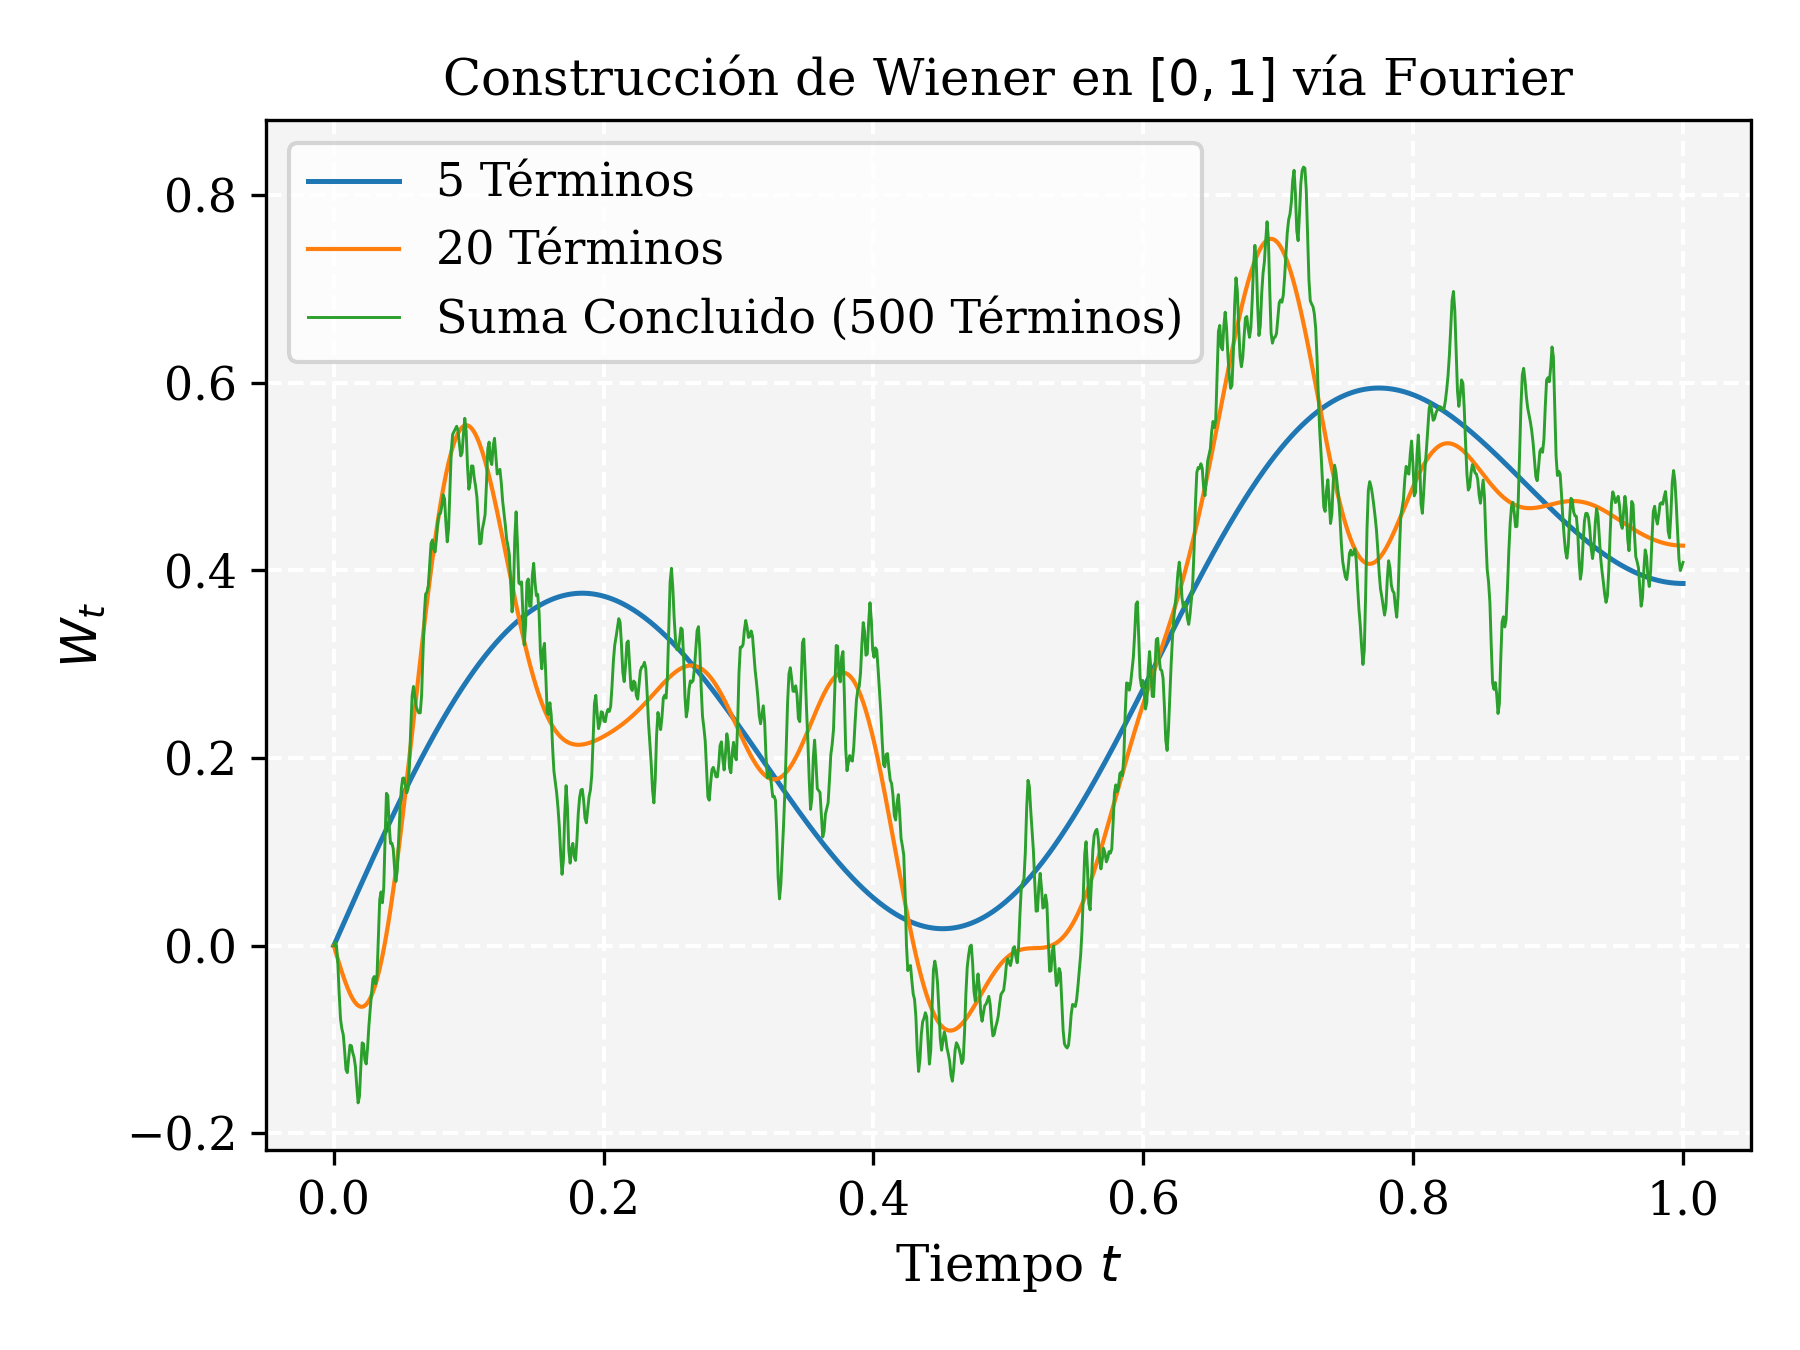
\includegraphics[width=0.75\textwidth]{wiener_fourier_construction.png}
    \caption{Simulación de la convergencia uniforme de la serie de Fourier de Wiener en el intervalo $[0,1]$.}
    \label{fig:wiener_fourier}
\end{figure}

\textbf{Descripción de la simulación de la construcción de Wiener:} \\
La simulación gráfica expuesta en la Figura \ref{fig:wiener_fourier} ilustra de manera empírica la descomposición armónica estocástica del proceso. En ella se aprecia el efecto de la acumulación de frecuencias: con una cantidad pequeña de términos ($N=5$), la trayectoria mantiene un perfil de onda trigonométrica completamente suave y diferenciable. Al incrementar los armónicos a $N=20$, comienzan a manifestarse perturbaciones locales en escalas más cortas. Finalmente, al incorporar $N=500$ términos, la serie converge hacia el comportamiento continuo pero rugoso e irregular intrínseco del movimiento browniano, demostrando analíticamente que el proceso carece de derivada en cualquier punto debido a su geometría puramente fractal.

\subsection{Visualización de la Ley del Logaritmo Iterado}
Para verificar de forma empírica el Teorema de Khinchin, se simuló una trayectoria Browniana continua sobre un horizonte temporal extendido de $t\in[0,2000]$. En la Figura 2 se grafica la trayectoria frente a las fronteras superiores e inferiores teóricas dadas por $\pm\sqrt{2t~log~log~t}.$ Se observa con total claridad matemática cómo la curva azul fluctúa de manera salvaje pero permanece estrictamente confinada dentro de la envoltura roja asintótica, tocando sus límites en repetidas ocasiones pero sin rebasarlos de manera permanente, validando de forma contundente que el límite superior del cociente es idénticamente 1.

\begin{figure}[htbp]
    \centering
    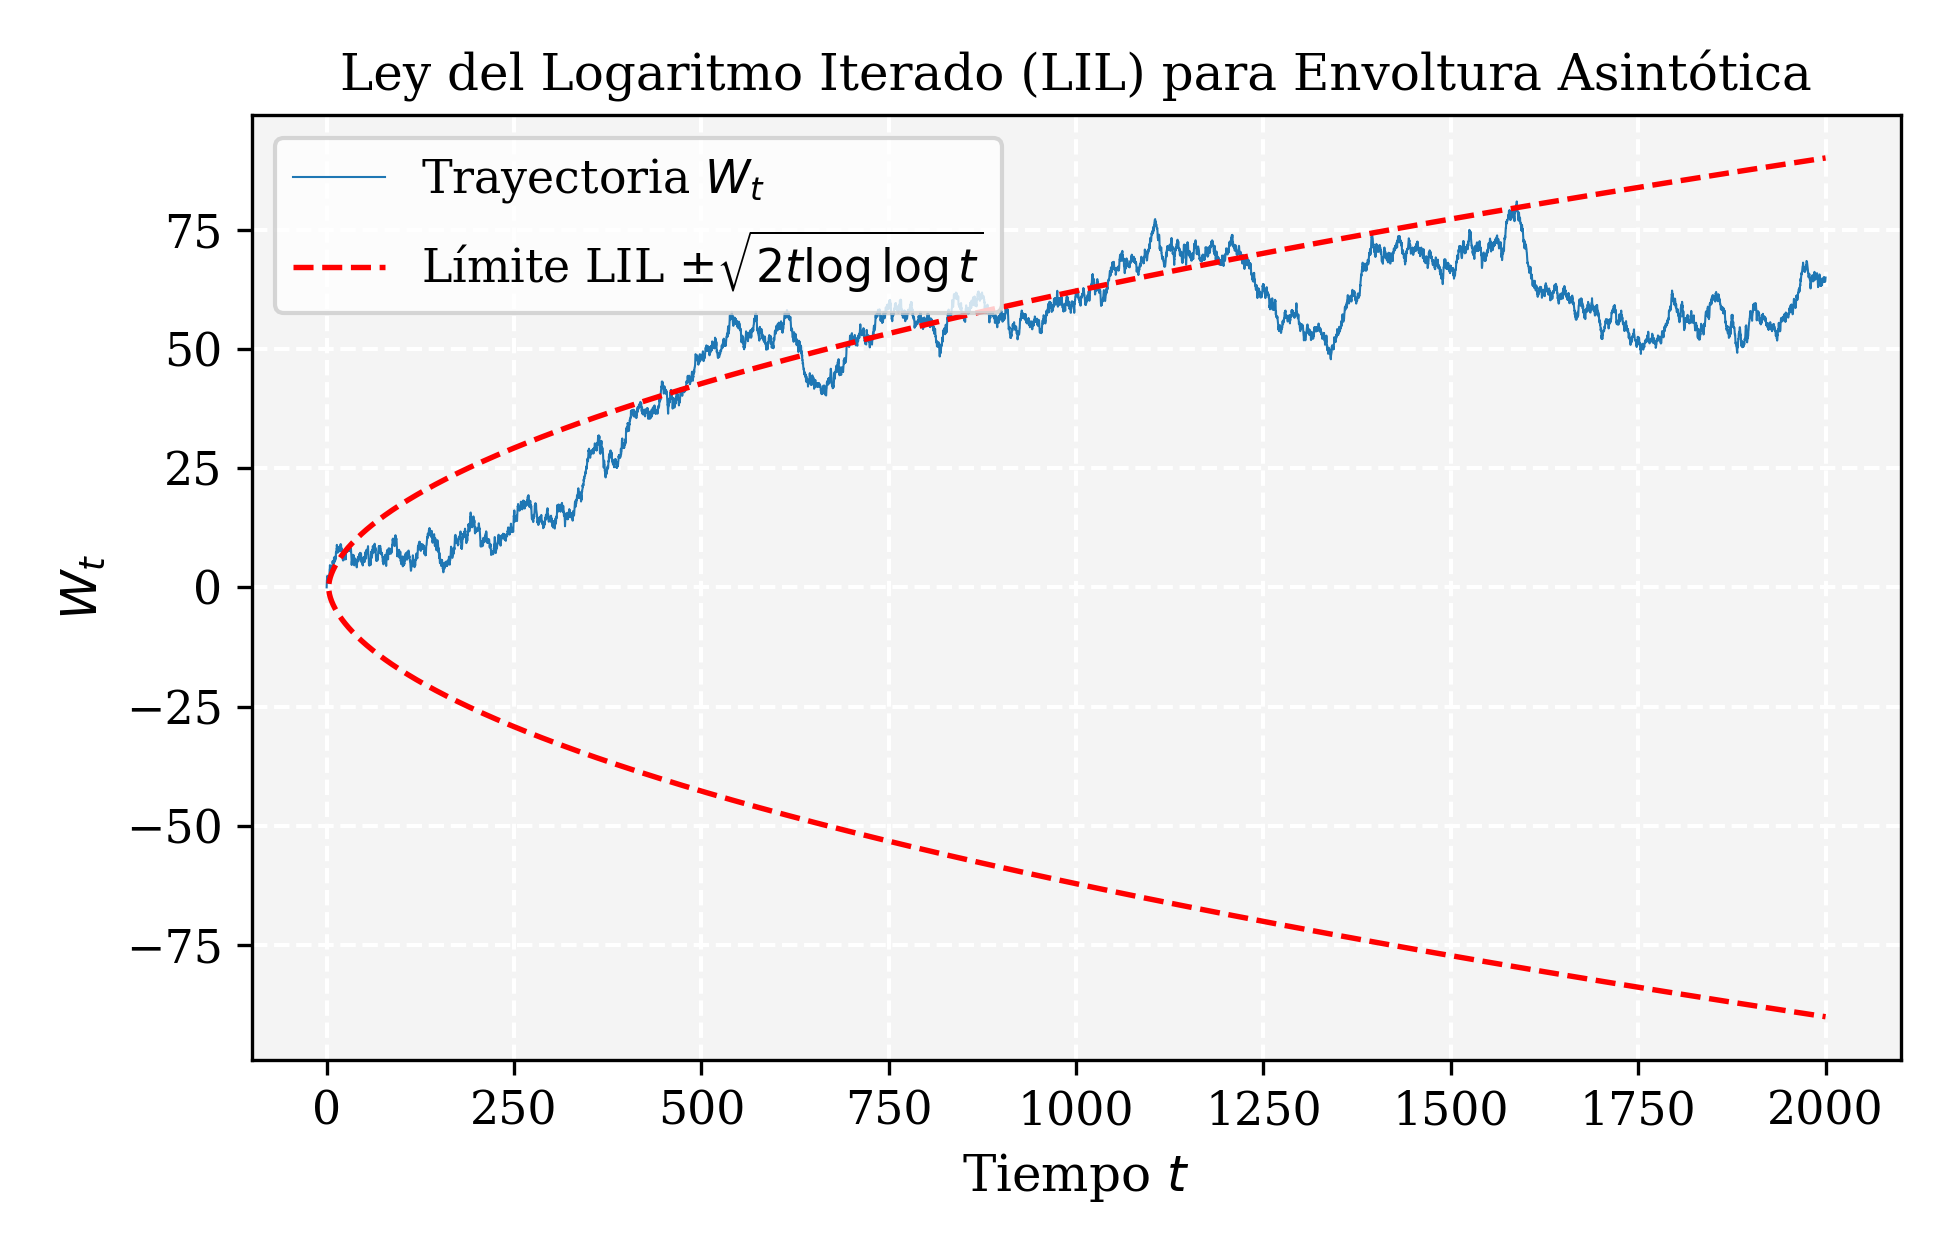
\includegraphics[width=0.75\textwidth]{lil_envelope_plot.png}
    \caption{Validación de la Ley del Logaritmo Iterado de Khinchin actuando como cota asintótica estricta.}
    \label{fig:lil_envelope}
\end{figure}

\textbf{Descripción de la simulación de la ley del logaritmo iterado:} \\
La simulación temporal de horizonte extendido plasmada en la Figura \ref{fig:lil_envelope} verifica experimentalmente los límites deterministas descubiertos por Khinchin. La curva azul representa el desplazamiento continuo e irregular del proceso de Wiener, el cual exhibe una fluctuación estadística salvaje. Sin embargo, al superponer las funciones de envoltura asintótica calculadas teóricamente mediante los términos $\pm\sqrt{2t \log \log t}$, se comprueba que el comportamiento extremo de la trayectoria queda confinado estrictamente dentro de estas barreras rojas discontinuas. El proceso alcanza y roza de forma recurrente dichos límites numéricos debido a la acumulación de probabilidad a largo plazo, pero es incapaz de superarlos de forma permanente, confirmando de manera sólida la validez analítica del teorema de Khinchin.


\section{Conclusión}

El movimiento browniano es uno de los objetos centrales de la teoría moderna de la probabilidad. Su origen físico permitió conectar fenómenos naturales con modelos matemáticos, mientras que su formalización abrió el camino para el estudio riguroso de procesos estocásticos continuos.

La construcción de Wiener mediante series de Fourier muestra que el movimiento browniano puede entenderse como una suma infinita de oscilaciones aleatorias. Esta idea es importante porque une el análisis matemático con la probabilidad, permitiendo construir trayectorias continuas pero altamente irregulares.

Por otra parte, la ley del logaritmo iterado, relacionada con los trabajos de Khinchin, revela que las fluctuaciones extremas del movimiento browniano obedecen una escala precisa. Aunque el proceso parece caótico, sus máximos y mínimos a largo plazo tienen un comportamiento matemáticamente determinado.

En conjunto, Fourier, Wiener y Khinchin permiten comprender el movimiento browniano desde distintas perspectivas. Fourier proporciona la herramienta analítica; Wiener construye el proceso de manera rigurosa; y Khinchin ayuda a describir el crecimiento extremo de sus fluctuaciones.

Por ello, el movimiento browniano no debe entenderse únicamente como un movimiento aleatorio, sino como una estructura matemática profunda donde convergen la física, el análisis, la probabilidad y la teoría de procesos estocásticos.

\section{Referencias}

\begin{thebibliography}{9}

\bibitem{peres}
Peres, Y. 
\textit{Some highlights from the history of probability}. 
Video de YouTube.

\bibitem{wiener}
Wiener, N. 
\textit{Differential-space}. 
Journal of Mathematics and Physics, 2, 131--174, 1923.

\bibitem{khinchin}
Khinchin, A. Y. 
\textit{Mathematical Foundations of Statistical Mechanics}. 
Dover Publications.

\bibitem{karatzas}
Karatzas, I., \& Shreve, S. E. 
\textit{Brownian Motion and Stochastic Calculus}. 
Springer.

\bibitem{durrett}
Durrett, R. 
\textit{Probability: Theory and Examples}. 
Cambridge University Press.

\bibitem{oksendal}
Oksendal, B. 
\textit{Stochastic Differential Equations: An Introduction with Applications}. 
Springer.

\end{thebibliography}

\end{document}